\chapter{Ratioed logic}
Ratiohead logic means that the characteristics of the circuit (statics and dynamics) depends on the ratio between the pull-up and the pull-down network.\\
This type of circuits the advantage of being less area consuming and with small output capacitance.\\

\section{Pseudo-NMOS}
The basic idea behind this logic is to use the same pull down network of an FC-CMOS implementation but using as pull up only a p-mos always on (with the gate grounded)

\centering
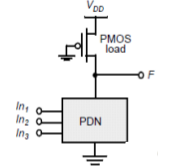
\includegraphics[width=0.35\textwidth]{C7_1.png}\\
\raggedright
       		
Obviously to pull down the output node the pull down network have to be stronger than the p-mos.\\
We drastically reduced the number of transistors form 2N+1 of the FC-CMOS logic to N+1 and doing so also the input and output capacitance.\\

\subsection{Static characteristics}
Let's take as example the pseudo-NMOS inverter

\centering
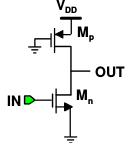
\includegraphics[width=0.2\textwidth]{C7_2.png}\\
\raggedright

$V_{OH}$ remains at VDD but $V_{OL}$ isn't at 0V since both transistors are on when the pull-down network is enabled.\\
Therefore we can estimate that $V_{OL}$ it's close to ground so we can found it's value supposing the pmos in velocity saturation and the nmos in ohmic region and comparing the currents when the input is at VDD and out at $V_{OL}$
\begin{equation}
k'_n \left(\frac{W}{L}\right)_n   V_{OL}(V_{DD}-V_{tn}-\frac{V_{OL}}{2})=k'_n \frac{W}{L}|_p V_{satp}(V_{DD}-V_{tp}-\frac{V_{satp}}{2})
\end{equation}
$V_{OL}$ stricktly depends on the relative ratio between nmos and pmos. Weaker pmos smaller the output voltage low.\\

\vspace{5mm}

Regarding the switching threshold we can suppose it's near the middle and write the ballance of currents with both transistors in velocity saturation where we find the term $V_M$ only in the nmos current
\begin{equation}
k'_n \left(\frac{W}{L}\right)_n  V_{satn}(V_{M}-V_{tn}-\frac{V_{satn}}{2})=k'_n \left(\frac{W}{L}\right)_p V_{satp}(V_{DD}-V_{tp}-\frac{V_{satp}}{2})
\end{equation}
then after getting the first value we can verify if our supposion was right and iterate.\\

\vspace{5mm}

Main drawback of this technology is the static power consumption that we have in correspondance of a logic 0.\\
This power can be evaluated as 
\begin{equation}
P_{static}=P(0)V_{DD}\cdot k'_n \left(\frac{W}{L}\right)_p V_{satp}(V_{DD}-V_{tp}-\frac{V_{satp}}{2})(1+\gamma_p(V_{DD}-V_{OL}))
\end{equation}

\subsection{Dynamic characteristics}

The intrinsic propagation delay can be evaluated in the same way as the FC-CMOS logic restoring the idea of equivalent resistance.\\
In the pull-up time we have to consider that it's an overestimation since we don't start from 0V but from $V_{OL}$.\\
In the pull-down time we're doing an underestimation since the pmos is on and try to charge the capacitance. In order to take into account this effect we can consider the pull-down resistance as
\begin{equation}
R_{pull-down}=\frac{R_{eq,n}}{1-\frac{R_{eq,n}}{R_{eq,p}}}
\end{equation}
Hidden in this relation there is the fact that if the pmos is too strong we aren't able to pull down the y node (for $R_n<R_p$, $R_{pd}$ becomes negative).\\

\vspace{5mm}

There is a trade off between static and dinamic proprieties as the following scheme shows

\centering
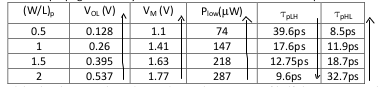
\includegraphics[width=0.5\textwidth]{C7_3.png}\\
\raggedright





\section{DCVSL}
This technology is an improvement of the pseudo-NMOS logic that eliminates the problem of static power consumption and makes the $V_{OL}=0$ using a positive feedback and a differential structure.\\
The basic structure is shown in figure 

\vspace{2mm}
\centering
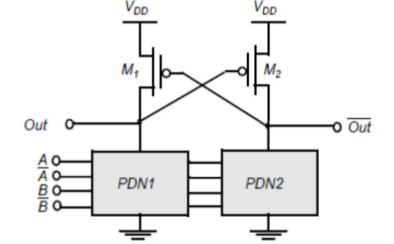
\includegraphics[width=0.35\textwidth]{C7_4.png}\\
\raggedright
\vspace{2mm}

The two pull-down network are complementary and we have a differential output.\\
At steady state there is no conductive path between the voltage supply and ground and the low output voltage is restored due to the feedback loop.\\
Although the logic is still ratioed since if the pull down network is not stronger than the PMOS transistor, the corresponding output node cannot be driven low.\\

\vspace{5mm}

This logics has still some problems since we have cross-conduction current the switching activity is increased ($\alpha_{sw}\simeq 1$) and the cross-connection between the two pmos as the differential naure can be troublesome.\\
















